\documentclass{magnolia}

\magtex{tex_driver={pdftex}}
\magfiche{document_nom={Graphe},
          auteur_nom={François Fayard},
          auteur_mail={francois.fayard@auxlazaristeslasalle.fr}}
\magexos{exos_matiere={maths},
         exos_niveau={mpsi},
         exos_chapitre_numero={8},
         exos_theme={Graphe}}
\magmisenpage{}
\maglieudiff{}
\magprocess

\begin{document}

%BEGIN_BOOK
\magsection{Graphes}

\exercice{nom={Graphe}}
Dessiner tous les graphes non orientés ayant exactement trois sommets.

\exercice{nom={Graphe}}
Combinen y a-t-il de graphes orientés ayant exactement trois sommets~? On ne demande pas de
les dessiner tous, mais uniquement de les dénombrer.

\exercice{nom={Afficher un graphe}}
\begin{questions}
\question Écrire une fonction \verb!afficheGraphe(g)! prenant en paramètre une liste
  d'adjacence $g$ et affichant le graphe sous la forme suivante
\begin{pythoncode}
0 -> 1 3
1 -> 2 3
2 -> 3
3 -> 1
\end{pythoncode}
  c'est-à-dire une ligne par sommet, avec pour chacun la liste de ses voisins.
\question Faire de même si $g$ est représenté par une matrice d'adjacence.
\end{questions}

\exercice{nom={Parcours en profondeur}}
Dérouler à la main le parcours en profondeur sur le graphe suivant
\begin{center}
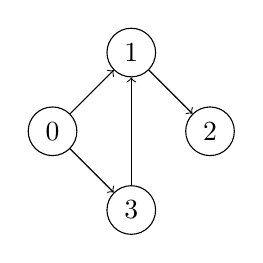
\begin{tikzpicture}
	\node[shape=circle,draw=black] (0) at (0,0) {0};
	\node[shape=circle,draw=black] (1) at (1,1) {1};
	\node[shape=circle,draw=black] (3) at (1,-1) {3};
	\node[shape=circle,draw=black] (2) at (2,0) {2};

	\path [->](0) edge node[left] {} (1);
	\path [->](0) edge node[left] {} (3);
	\path [->](3) edge node[left] {} (1);
	\path [->](1) edge node[left] {} (2);
\end{tikzpicture}
\end{center}
pour différentes valeurs du sommet de départ. Donner à chaque fois la valeur finale pour
l'ensemble de sommets \verb!vus!, c'est-à-dire l'ensemble des sommets atteints par le parcours.

\exercice{nom={Parcours en largeur}}
Dérouler à la main le parcours en largeur sur le graphe suivant
\begin{center}
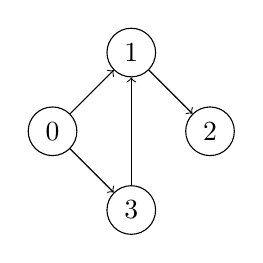
\begin{tikzpicture}
	\node[shape=circle,draw=black] (0) at (0,0) {0};
	\node[shape=circle,draw=black] (1) at (1,1) {1};
	\node[shape=circle,draw=black] (3) at (1,-1) {3};
	\node[shape=circle,draw=black] (2) at (2,0) {2};

	\path [->](0) edge node[left] {} (1);
	\path [->](0) edge node[left] {} (3);
	\path [->](3) edge node[left] {} (1);
	\path [->](1) edge node[left] {} (2);
\end{tikzpicture}
\end{center}
pour différentes valeurs du sommet de départ. Donner à chaque fois la valeur finale pour
l'ensemble \verb!dist!, c'est-à-dire la distance à la source de chaque sommet atteint par
le parcours.

% \exercice{nom={Coloriage glouton d'un graphe}}

%END_BOOK

\end{document}
